\section{Introduction}

\begin{figure}[t]
\centering
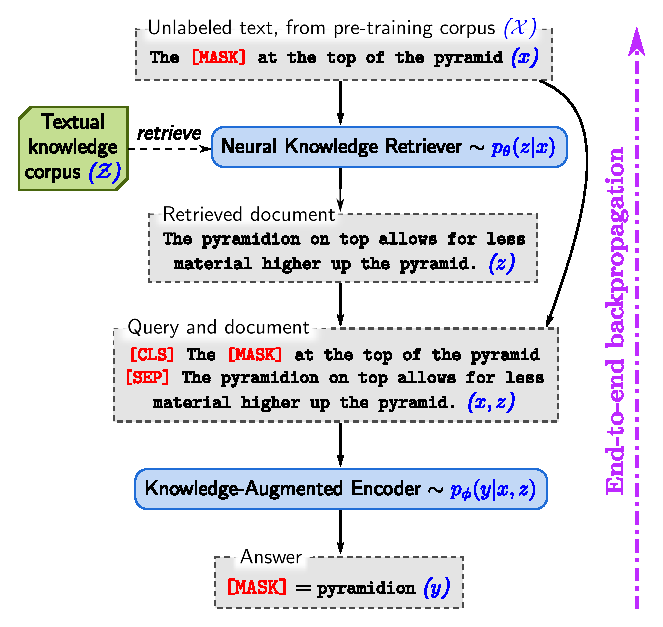
\includegraphics[width=\columnwidth]{figures/intro_end_to_end.eps}
\caption{\label{fig:intro} \ \thename augments language model pre-training with a {\bf neural knowledge retriever}
that retrieves knowledge from a {\bf textual knowledge corpus}, $\cZ$ (e.g., all of Wikipedia). Signal from the language modeling objective backpropagates all the way through the retriever, which must consider millions of documents in $\cZ$---a significant computational challenge that we address.}
\end{figure}

Recent advances in language model pre-training have shown that models such as BERT~\cite{bert}, RoBERTa~\cite{roberta} and T5~\cite{t5} store a surprising amount of world knowledge,
acquired from the massive text corpora they are trained on~\cite{lm_as_kb}.
For example, BERT is able to correctly predict the missing word in the following sentence:
\nl{The \blank\xspace is the currency of the United Kingdom} (answer: \nl{pound}).

In these language models, the learned world knowledge is stored {\em implicitly} in the parameters of the underlying neural network. This makes it difficult to determine what knowledge is stored in the network and where.
Furthermore, storage space is limited by the size of the network---to capture more world knowledge, one must train ever-larger networks, which can be prohibitively slow or expensive. 

To capture knowledge in a more interpretable and modular way, we propose a novel framework, \thefullname (\thename) pre-training, which augments language model pre-training algorithms with a learned {\em textual knowledge retriever}.
In contrast to models that store knowledge in their parameters, this approach \emph{explicitly} exposes the role of world knowledge by asking the model to decide what knowledge to retrieve and use during inference.
Before making each prediction, the language model uses the retriever to retrieve documents\footnotemark~from a large corpus such as Wikipedia,
% THE FOOTNOTE IS AT THE END TO COMBINE WITH THE RIGHT COLUMN
and then attends over those documents to help inform its prediction.
Learning this model end-to-end requires backpropagating through a retrieval step that considers an entire corpus of textual knowledge, as shown in Figure~\ref{fig:intro}.

The key intuition of \thename is to
train the retriever using a {\em performance-based} signal from unsupervised text:
a retrieval that {\em improves} the language model's perplexity is helpful and should be rewarded, while an uninformative retrieval should be penalized. 
For example, in Figure~\ref{fig:intro}, if the model needs to fill the blank in \nl{the~\blank~at the top of the pyramid}, the retriever should be rewarded for selecting a document containing \nl{The pyramidion on top allows for less material higher up the pyramid}. We achieve this behavior by modeling our {\em retrieve-then-predict} approach as a latent variable language model and optimizing the marginal likelihood.

Incorporating a large-scale neural retrieval module
during pre-training constitutes a significant computational challenge, %for pre-training,
since the retriever must consider millions of candidate documents for each pre-training step, and we must backpropagate through its decisions. To address this, we structure the retriever such that the computation performed for each document can be cached and asynchronously updated, and selection of the best documents can be formulated as Maximum Inner Product Search (MIPS).

Numerous prior works have
demonstrated the benefit of adding a discrete retrieval step to neural networks~\cite{key_value_memorynetwork, drqa}, but did not apply the framework
to language model pre-training and employed non-learned retrievers to handle large-scale document collections.
In the language modeling literature, the $k$-Nearest Neighbor Language Model~\cite{knnlm} ($k$NN-LM) retrieves similar LM examples to improve memorization. However, $k$NN-LM was not fine-tuned for downstream tasks, perhaps because it is unclear how to adapt the retrieval mechanism: a $k$NN can only use examples labeled for the target task---during fine-tuning, this precludes LM examples, which contain the desired world knowledge. In contrast, \thename's retriever is designed to transfer to other tasks, and the retrieval is just text, not a labeled example.

We evaluate our approach by fine-tuning the models pre-trained with \thename on the task of Open-domain Question Answering (\openqa), one of the most knowledge-intensive tasks in natural language processing.
%
We evaluate on three popular \openqa benchmarks (\nq, \wq, and \trec) and compare to state-of-the-art \openqa models, including both extremely large models that store knowledge implicitly (such as T5) as well as previous approaches that also use a knowledge retriever to access external knowledge, but implement retrieval in a more heuristic fashion~\cite{orqa,openqa_hardem,rrp_salesforce}. \thename achieves new state-of-the-art results on all three benchmarks, significantly outperforming all previous systems by 4-16\% absolute accuracy. We also demonstrate qualitative benefits of \thename, including interpretability and modularity.

\footnotetext{We use the term ``document'' loosely to refer to a passage from the knowledge corpus, not necessarily a whole article.}